\documentclass[a4paper]{article}

\usepackage[margin=1in]{geometry} 
\usepackage{amsmath,amsthm,amssymb}
\usepackage{amssymb}
\usepackage{float}
\usepackage{graphicx}
\usepackage{xcolor}
\usepackage[UKenglish]{isodate}
\origdate
\cleanlookdateon
\usepackage[utf8]{inputenc}
\usepackage[hidelinks]{hyperref}
\usepackage{tikz-cd}
\usepackage{enumitem}
\usepackage{mathtools}
\usepackage{pgfplots}
\usepackage{float}
\usepackage{tikz, venndiagram}
\usepackage{tkz-euclide}
\usepackage{tabu}
\renewcommand{\baselinestretch}{1.5} 

%%% Better lambda 
\usepackage{pifont}
\makeatletter
\newcommand\Pimathsymbol[3][\mathord]{%
  #1{\@Pimathsymbol{#2}{#3}}}
\def\@Pimathsymbol#1#2{\mathchoice
  {\@Pim@thsymbol{#1}{#2}\tf@size}
  {\@Pim@thsymbol{#1}{#2}\tf@size}
  {\@Pim@thsymbol{#1}{#2}\sf@size}
  {\@Pim@thsymbol{#1}{#2}\ssf@size}}
\def\@Pim@thsymbol#1#2#3{%
  \mbox{\fontsize{#3}{#3}\Pisymbol{#1}{#2}}}
\makeatother
% the next two lines are needed to avoid LaTeX substituting upright from another font
\input{utxmia.fd}
\DeclareFontShape{U}{txmia}{m}{n}{<->ssub * txmia/m/it}{}
% you may also want
\DeclareFontShape{U}{txmia}{bx}{n}{<->ssub * txmia/bx/it}{}
% just in case
%\DeclareFontShape{U}{txmia}{l}{n}{<->ssub * txmia/l/it}{}
%\DeclareFontShape{U}{txmia}{b}{n}{<->ssub * txmia/b/it}{}
% plus info from Alan Munn at https://tex.stackexchange.com/questions/290165/how-do-i-get-a-nicer-lambda?noredirect=1#comment702120_290165
\newcommand{\pilambdaup}{\Pimathsymbol[\mathord]{txmia}{21}}
\pgfplotsset{compat=1.16}
\begin{document}
\title{Notes on Probability and Statistics\\[0.1cm]
    \large 30.003 Probability and Statistics, Term 4 2019}
\author{Wei Min Cher}
\date{05 Jan 2020}

\maketitle

\tableofcontents

\newpage
\section{W1: Probability and Statistics}
\subsection{Definitions}
\begin{itemize}
    \item Population: well defined collection of objects
    \item Sample: subset of population selected in certain manner
    \item Variable: any characteristic whose value may change from one object to another in population
    \newline
    \item Probability: properties of populations known, question regarding sample taken from population are investigated \textbf{(deductive reasoning)}
    \item Statistics: characteristics of sample known from experiments, conclusions regarding population are made \textbf{(inductive reasoning)}
\end{itemize}
\begin{center}
    \begin{tikzcd}
    \text{Population} \arrow[r, bend left=45, "\text{Probability}"{name=U, above}]
    & \text{Sample} \arrow[l, bend left=45, "\text{Statistics}"{name=D}]
    \end{tikzcd}
\end{center}
\begin{itemize}
    \item Descriptive statistics: techniques to describe a sample/population
    \item Inferential statistics: making predictions or inferences about population from observations and analyses of sample
\end{itemize}
\subsection{Frequency} 
\begin{itemize}
    \item Frequency: number of times value occurs in data set
    \item Relative frequency: fraction or proportion of times the value occurs
\end{itemize}
\subsection{Range and mean}
\begin{itemize}
    \item Range: difference between largest and smallest sample values
    \item Mean: average of all values
    \newline
    \item Population mean is denoted by $\mu$
    \item Sample mean is denoted by $\Bar{x}$, where $$\Bar{x} = \frac{\sum x_{i}}{n}, \text{ and $n$ denoting the number of data points}$$
\end{itemize}
\subsection{Variance and standard deviation}
\begin{itemize}
    \item Variance: measures variability of data set
    \item Population variance is denoted by $\sigma^2$, where
    $$\sigma^2 = \frac{1}{N}\sum_{i=1}^{N}\left(x_{i}-\mu\right)^{2}, \text{ and $N$ denoting the size of the population}$$
    \item Sample variance is denoted by $s^2$, where
    $$s^2 = \frac{1}{n-1}\sum_{i=1}^{n}\left(x_{i}-\Bar{x}\right)^2, \text{ and $n$ denoting the size of the sample}$$
    \newline
    \item Standard deviation is denoted as $\sigma$ for population variance and $s$ for sample variance, and is calculated either by:
    $$\sigma = \sqrt{\sigma^2}, \text{ or } s = \sqrt{s^2}$$
    where $\sigma^2$ is the population variance and $s^2$ is the sample variance
    \begin{itemize}[label=$\circ$]
        \item Shortcut to calculate population variance:
        $$\sigma^2 = \frac{1}{N}\sum_{i=1}^{N}x_{i}^{2}-\mu^2$$
    \end{itemize}
\end{itemize}
\subsection{Linear transformation of sample}
Let $x_{1}, x_{2}, \ldots, x_{n}$ be a sample, with $a$ and $b$ being constants. If $y_{i} = ax_{i}+b$ is a linear transformation of $x_{i}$ for $i = 1, 2, \ldots, n$, then 
\begin{align*}
    \Bar{y} &= a\Bar{x}+b\\
    s_{y}^2 &= a^{2}s_{x}^{2}
\end{align*}
\subsection{Median}
\begin{itemize}
    \item Median: the middle value in a data set
    \item Population median $\tilde \mu$
    $$\tilde \mu = \begin{dcases*} \quad x_{m}\vphantom{\frac{0}{0}}&
  $N$ odd, $m = \frac{N+1}{2}$;\\
\quad \frac{x_{m} + x_{m+1}}{2} & $N$ even, $m = \frac{N}{2}$;
    \end{dcases*}$$
    \item Sample median $\tilde x$
    $$\tilde x = \begin{dcases*} \quad x_{m}\vphantom{\frac{0}{0}}&
  $n$ odd, $m = \frac{n+1}{2}$;\\
\quad \frac{x_{m} + x_{m+1}}{2} & $n$ even, $m = \frac{n}{2}$;
    \end{dcases*}$$
\end{itemize}
\subsection{Percentage and percentile}
\begin{itemize}
    \item Percentage: number specifying proportion
    \item Percentile
    \begin{itemize}[label=$\circ$]
        \item value below which a given percentage of observations falls
        \item data set is ordered as $x_{1}' \leq x_{2}'\leq \cdots \leq x_{n}'$,\\ where $x_{1}'$ and $x_{n}'$ are the smallest and largest data values respectively
        \item $x_{i}'$ corresponds to the $\frac{100(i-0.5)}{n}$th percentile
    \end{itemize}
\end{itemize}
\subsection{Histogram}
\begin{itemize}
    \item A graphical representation of the distribution of data
\end{itemize}
\mbox{}
\begin{center}
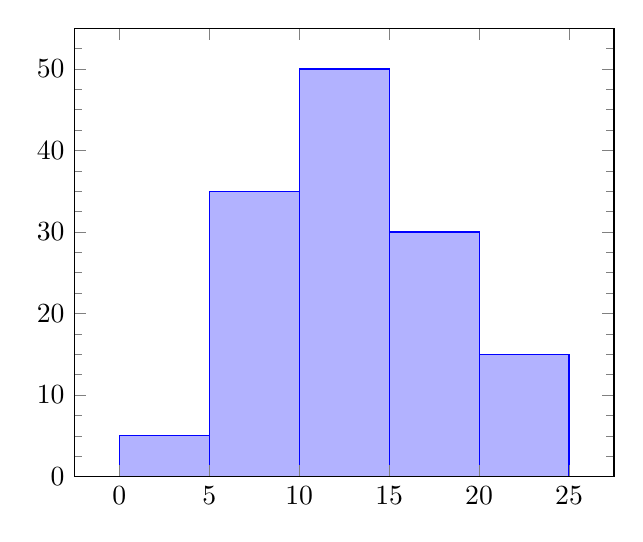
\begin{tikzpicture}
\begin{axis}[
    ymin=0, ymax=55,
    minor y tick num = 3,
    area style,
    ]
\addplot+[ybar interval,mark=no] plot coordinates { (0, 5) (5, 35) (10, 50) (15, 30) (20, 15) (25, 0) };
\end{axis}
\end{tikzpicture}
\end{center}
\subsection{Sample space and events}
\begin{itemize}
    \item Sample space: the set of all possible outcomes of an experiment
    \begin{enumerate}
        \item Collectively exhaustive
        \begin{itemize}[label=$\circ$]
            \item Contain all possible outcomes
        \end{itemize}
        \item Mutually exclusive
        \begin{itemize}[label=$\circ$]
            \item Each outcome in sample space should be unique
        \end{itemize}
    \end{enumerate}
    \item Event: collection of outcomes contained in sample space $\Omega$
    \begin{enumerate}
        \item Simple event: exactly one outcome e.g. \textit{value of die rolled}
        \item Compound event: \textgreater \ 1 outcome e.g. \textit{event that outcome is even}
    \end{enumerate}
\end{itemize}
\subsection{Sample Space vs Population}
\begin{itemize}
    \item Sample space: contains mutually exclusive events
    \item Population: events can repeat many times
\end{itemize}
\subsection{Set Theory}
\begin{itemize}
    \item Complement of event A, $A^c$: set if outcomes in $\Omega$ that are not in A
    \item Intersection of 2 events A and B, $A\cap B$: all outcomes that are in A and B
    \item Union of 2 events A and B, $A\cup B$: all outcomes that are either in A or B
    \item Null event, $\varnothing$: event with no outcome
    \newline
    \item Events A and B are mutually exclusive/disjoint if $A\cap B = \varnothing$
    \item Events $A_{1}, A_{2}, A_{3}, \ldots$ are mutually exclusive (or pairwise disjoint) if no 2 events have any outcome in common
\end{itemize}
\subsection{De Morgan's Laws}
\begin{align*}
    (A\cup B)^{c} &= A^{c} \cap B^{c}\\
    (A\cap B)^{c} &= A^{c} \cup B^{c}\\
    A \cup B &= A+B-A\cap B
\end{align*}
\begin{itemize}
    \item P(A): probability that event A will occur
\end{itemize}
\subsection{Axiom of Probability}
\begin{enumerate}
    \item For any event A, P(A) $\leq$ 0.
    \item P($\Omega$) = 1
    \item Any infinite collection of mutually exclusive/disjoint events $A_{1}, A_{2}, A_{3}, \ldots, A_{n}$ satisfies
    $$P(A_{1}\cup A_{2}\cup A_{3} \cup \ldots \cup A_{n}) = \sum_{i=1}^{\infty}P(A_{i})$$
\end{enumerate}
\subsection{Properties of Probability}
\begin{itemize}
    \item For any event A, $P(A) + P(A^c) = 1$ \textbf{OR} $P(A) = 1 - P(A^c)$.
    \item $P(\Omega) = P(A\cup A^c) = P(A) + P(A^c)$\\
    $\because$ \ $A$ \text{and} $A^c$ are disjoint
    \item For any event A, $P(A) \leq 1$.
    \item For a null event $\varnothing$, $P(\varnothing) = 0$
    \begin{itemize}[label=$\circ$]
        \item Does \textbf{NOT} suggest A = $\varnothing$
    \end{itemize}
    \item Similarly, P(A) = 1 does \textbf{NOT} suggest A = $\Omega$
\end{itemize}
\subsection{Equally likely outcomes}
$$P(\text{equally likely event}) = \frac{1}{n},\text{ where n is the number of equally likely events}$$
\subsection{Simple and compound events}
\begin{itemize}
    \item Simple event: Find out how many outcomes in sample space
    \item Compound event: Find out how many outcomes in event
\end{itemize}
\newpage
\section{W1: Counting Technique}
\subsection{Finding probability}
\begin{itemize}
    \item Computing probability $\rightarrow{}$ counting
    $$P(A) = \frac{N(A)}{N}$$
    \begin{itemize}[label=$\circ$]
        \item where $N(A)$ is the number of outcomes for event A, \\and $N$ is the number of outcomes in the sample space  
    \end{itemize}
\end{itemize}
\subsection{Tuple}
\begin{itemize}
    \item Group of $k$ elements: k-tuple
    \item The 1\textsuperscript{st} element is selected in $n_1$ ways;
    the 2\textsuperscript{nd} element is selected in $n_2$ ways; the k\textsuperscript{th} element is selected in $n_k$ ways; such that \textit{the elements are selected independently}.
\end{itemize}
\subsection{Permutation}
\begin{itemize}
    \item Ordered subset
    \item Number of permutations of size $k$ formed from $n$ objects:
    $$P_{k, n} = \frac{n!}{(n-k)!}$$
\end{itemize}
\subsection{Combination}
\begin{itemize}
    \item Unordered subset of a group
    \item Number of combinations of size $k$ formed from $n$ objects:
    $$\binom{n}{k} \text{ or }C_{k, n} = \frac{P_{k, n}}{k!} = \frac{n!}{k!(n-k)!}$$
    \item Disregards the different outcomes due to order
\end{itemize}
\newpage
\section{W2: Conditional Probability}
\begin{itemize}
    \item Probability of event A given that event B has occurred: P(A$\mid$B)
    $$P(A\mid B) = \frac{P(A\cap B)}{P(B)}$$
\end{itemize}
\begin{center}
    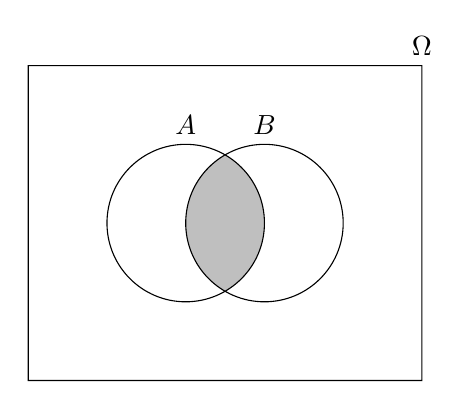
\begin{tikzpicture}
\scope % A \cap B
\clip (0,0) circle (1);
\fill[lightgray] (1,0) circle (1);
\endscope
% outline
\draw (0,0) circle (1) (0,1) node [text=black,above] {$A$}
      (1,0) circle (1) (1,1) node [text=black,above] {$B$}
      (-2,-2) rectangle (3,2) node [text=black,above] {$\Omega$};
\end{tikzpicture}
\end{center}
\subsection{Law of Total Probability}
\begin{itemize}
    \item Events $A_{1}, A_{2}, \ldots, A_{k}$ are exhaustive if one $A_{i}$ must occur, i.e. $A_{1}\cup A_{2}\cup\ldots\cup A_{k} = \Omega$.
    \item Let $A_{1}, A_{2}, \ldots, A_{k}$ be mutually exclusive and exhaustive events.\\For any other event B,
    $$P(B) = \sum_{i=1}^{k}P(B\mid A_{i})P(A_{i})$$
\end{itemize}
\begin{center}
    \begin{venndiagram3sets}[labelA = $A_{1}$, labelB = $A_{2}$, labelC = $A_{3}$, labelABC = $B$]
    \fillACapB  
    \fillACapC
    \fillBCapC
    \fillACapCCapB
    \setpostvennhook{\draw (venn top right) node[text=black,above] {$\Omega$};}
    \end{venndiagram3sets}
\end{center}
\newpage
\subsection{Bayes' Theorem}
\begin{itemize}
    \item Let $A_{1}, A_{2}, \ldots, A_{k}$ be mutually exclusive and exhaustive events with prior unconditional \\probabilities $P(A_{i}), i = 1, 2, \ldots, k$
    \item For any other event B with P(B) \textgreater \  0, the conditional posterior probability of $A_{j}$ given that B has occurred is 
    \begin{align*}
        P(A_{j}\mid B) &= \frac{P(A_{j}\cap B)}{P(B)}\\
        &= \frac{P(B\cap A_{j})}{P(B)}\\
        &= \frac{P(B\mid A_{j})P(A_{j})}{\sum_{i=1}^{k}P(B\mid A_{i})P(A_{i})}
    \end{align*}
\end{itemize}
\subsection{Independence of Random Variables}
\begin{itemize}
    \item Independence: occurrence/non-occurrence of one event has no bearing\\ on the chance that the other will occur
    \begin{itemize}[label=$\circ$]
        \item $P(A\mid B) = P(A)$: A and B are independent
        \item $P(A\mid B) \neq P(A)$: A and B are not independent
    \end{itemize}
    \item Independence of A and B also implies $P(B\mid A) = P(B)$ if $P(A) > 0$
\end{itemize}
\subsubsection{Multiplication Rule}
\begin{itemize}
    \item A and B are independent iff. $P(A\cap B) = P(A)P(B)$
\end{itemize}
\subsubsection{Independence of several events}
\begin{itemize}
    \item Events $A_{1}, A_{2}, \ldots, A_{n}$ are mutually independent if for every $k \in \{2, 3, \ldots n\}$ and every subset of indices $i_{1}, i_{2}, \ldots, i_{k}$:
    $$P(A_{i1}\cap A_{i2}\cap\ldots\cap A_{ik}) = P(A_{i1})P(A_{i2})\ldots P(A_{ik})$$
    \item Events are mutually independent if probability of the intersection of any subset of the $n$ events is equal to the product of the individual probabilities.
\end{itemize}
\subsubsection{Disjoint and independent events}
\begin{itemize}
    \item Disjointness: set-theory concept
    \begin{itemize}[label=$\circ$]
        \item Sets of each group of outcomes share nothing in common
    \end{itemize}
    \item Independence: probability concept
    \begin{itemize}[label=$\circ$]
        \item Event is not influenced by the outcome of another event
    \end{itemize}
\end{itemize}
\newpage
\section{W2: Discrete Random Variable}
\subsection{Random Variable (RV)}
\begin{itemize}
    \item Random variable (RV): a variable depending on outcomes of a random phenomenon
    \item Discrete RV: possible values make up a finite set or "countable" in finite set
    \item Continuous RV: possible values make up an infinite set
    \item Bernoulli RV: any RV whose only possible values are 0 and 1
\end{itemize}
\subsection{Probability Mass Function (PMF) for Discrete RV}
\begin{itemize}
    \item Known as probability mass function (pmf)
    \begin{itemize}[label=$\circ$]
        \item e.g. $p(0) = \frac{1}{8}, \ p(1) = \frac{3}{8}, \ p(2) = \frac{3}{8}, \ p(3) = \frac{1}{8}$
    \end{itemize}
    \item Completely describes probabilistic properties of RV X
    \item For any pmf, $p(x)\leq 0$ and $\sum_{\text{all possible x}}p(x) = 1$
\end{itemize}
\subsection{Parameter of probability distribution}
\begin{itemize}
    \item Possible value(s) which p(x) depends on
    \item Different value(s) determine a different probability distribution
    \item Collection of all probability distributions for different parameters: \textit{family of probability distributions}
\end{itemize}
\subsection{Bernoulli RV}
\begin{itemize}
    \item pmf of any Bernoulli RV:
    $$p(x; \alpha) = \begin{cases}
    \quad 1-\alpha,&\mbox{if }x = 0\\
    \quad \alpha,&\mbox{if }x = 1\\
    \quad 0, &\mbox{otherwise}
    \end{cases}
    $$
    \item $\alpha$ is a parameter, where $0<\alpha<1$
    \item Each different value of $\alpha$ between 0 and 1 determines a different member of the Bernoulli family of distributions
\end{itemize}
\subsection{Bernoulli process}
\begin{itemize}
    \item A process with repeated independent trials
    \item 2 outcomes: 1 (success), 0 (failure)
    \item Success rate of trials is the same
\end{itemize}
\subsection{Binomial distribution}
\begin{itemize}
    \item pmf of binomial RV:
    $$p(x;n,p) = \begin{cases}
    \quad C_{x, n}p^{x}(1-p)^{n-x},&\mbox{}x = 0, 1, \ldots, n\\
    \quad 0, &\mbox{otherwise}
    \end{cases}
    $$
    \begin{itemize}[label=$\circ$]
        \item where $n$ is the number of trials, and $p$ is the success rate of each trial
    \end{itemize}
    \item Since $\sum_{\text{all possible x}}p(x) = 1$, 
    $$\sum_{x = 0}^{n}p(x;n,p) = \sum_{x = 0}^{n}C_{x, n}p^{x}(1-p)^{n-x} = 1$$
\end{itemize}
\subsection{Geometric distribution}
\begin{itemize}
    \item Probability distribution of number of Bernoulli trials $X$ needed to get 1 success
    \item If $X = x$, $x-1$ failures followed by success
    \item pmf of geometric RV:
    $$p(x) = \begin{cases}
    \quad p(1-p)^{x-1},&\mbox{}x = 1, 2, \ldots\\
    \quad 0, &\mbox{otherwise}
    \end{cases}
    $$
    \begin{itemize}[label=$\circ$]
        \item where $p$ is the success rate of each trial
    \end{itemize}
    \item Since $\sum_{\text{all possible x}}p(x) = 1$, 
    $$\sum_{x=1}^{\infty}p(1-p)^{x-1} = p\sum_{i=0}^{\infty}(1-p)^{i}=\frac{p}{1-(1-p)} = 1
    $$
\end{itemize}
\subsection{Poisson distribution}
\begin{itemize}
    \item Used to model the number of occurrences of events in a time interval,\\ where the average occurrence is $\pilambdaup$
    \item pmf of Poisson RV:
    $$
    p(x; \pilambdaup) = \begin{dcases*}
    \quad\frac{\pilambdaup^{x} e^{-\pilambdaup}}{x!},&$x$ = 0, 1, $\ldots$\\
    \quad0\vphantom{\frac{0}{0}}, & otherwise
    \end{dcases*}
    $$
    \begin{itemize}[label=$\circ$]
        \item where $\pilambdaup$ is the parameter of Poisson distribution
    \end{itemize}
    \item Since $\sum_{\text{all possible x}}p(x) = 1$, 
    $$\sum_{n=0}^{\infty} \frac{\pilambdaup^{x}e^{-\pilambdaup}}{x!} = e^{-\pilambdaup}\sum_{n=0}^{\infty}\frac{\pilambdaup^x}{x!}= e^{-\pilambdaup}e^{\pilambdaup} = 1
    $$
\end{itemize}
\subsection{Cumulative Distribution Function (CDF)}
\begin{itemize}
    \item CDF $F(x)$ of discrete RV $X$ with pmf $p(x):$
    $$F(x) = P(X\leq x) = \sum_{y: y\leq x}p(y)
    $$
    \item $F(x)$ is the probability that the observed value is at most $x$
    \item Graph of $F(x)$ for discrete RV $X$ is the linear combination of step functions, such that
    $$
    \lim_{x\to -\infty}F(x) = 0\text{ and }\lim_{x\to\infty}F(x) = 1
    $$
\end{itemize}
\newpage
\section{W3: Expectation}
\subsection{Expected Value}
\begin{itemize}
    \item Expected value $E(X)$
    $$E(X) = \mu_{x} = \sum_{x\in D}x\cdot p(x), \text{ provided that }\sum_{x \in D}|x|\cdot p(x) < \infty
    $$
    \item Expected value of a function $E[h(X)]$
    $$E[h(X)] = \mu_{h(x)} = \sum_{x\in D}h(x)\cdot p(x)
    $$
    \item Expected value of a linear function $aX + b$
    $$E(aX+b) = aE(X) + b
    $$
\end{itemize}
\subsection{Variance}
\begin{itemize}
    \item Variance $V(X)$
    \begin{center}
        $\begin{matrix}
        V(X) = \sum_{x\in D}(x-\mu)^{2}p(x) = E[(X-\mu)^2], \text{ provided that the expectation exists}\\
        \textbf{OR}\\
        \text{Population variance, }\sigma^2 = V(X) = E(X^2)-[E(X)]^2
        \end{matrix}$
    \end{center}
    \item Variance of a function $V[h(X)]$
    $$V[h(X)] = \sum_{x\in D}\{h(x)-[E(X)]\}^{2}\cdot p(x)
    $$
    \item Variance of a linear function $aX + b$
    \begin{align*}
        V(aX + b) &= a^{2}V(X)\\
        \sigma_{aX+b} &= |a|\sigma_{x}
    \end{align*}
\end{itemize}
\subsection{Expected Value and Variance of Discrete PMFs}
\subsubsection{Bernoulli RV}
\paragraph{Expected value $E(X)$}
\begin{align*}
    E(X) &= \sum_{x\in D}x\cdot p(x)\\
    &= 0(1-p)+1(p)\\
    &= p
\end{align*}
\paragraph{Variance $V(X)$}
\begin{align*}
    V(X) &= E(X^2)-[E(X)]^2\\
    &= 0^2(1-p)+1^2(p)-p^2\\
    &= p-p^2\\
    &= p(1-p)
\end{align*}
\subsubsection{Binomial RV}
The complete proof for expected value and variance can be found here:\\ \href{https://www.math.ubc.ca/~feldman/m302/binomial.pdf}{https://www.math.ubc.ca/$\sim$feldman/m302/binomial.pdf}
\paragraph{Expected value $E(X)$}
$$E(X) = np$$
\paragraph{Variance $V(X)$}
$$V(X) = np(1-p)$$
\subsubsection{Geometric RV}
The complete proof for expected value and variance can be found here:\\
\href{https://semath.info/src/st-geometric-distribution.html}{https://semath.info/src/st-geometric-distribution.html}
\paragraph{Expected value $E(X)$}
$$E(X) = \frac{1}{p}$$
\paragraph{Variance $V(X)$}
$$V(X) = \frac{1-p}{p^2}$$
\subsubsection{Poisson RV}
The complete proof for expected value and variance can be found here:\\
\href{https://www.statlect.com/probability-distributions/Poisson-distribution}{https://www.statlect.com/probability-distributions/Poisson-distribution}
\paragraph{Expected value $E(X)$}
$$E(X) = \pilambdaup$$
\paragraph{Variance $V(X)$}
$$V(X) = \pilambdaup$$
\newpage
\section{W3: Continuous Random Variable}
\subsection{Definition}
\begin{itemize}
    \item Continuous RVs can take on any value in a continuous range (e.g. real numbers)
    \begin{itemize}[label=$\circ$]
        \item In contrast, discrete RVs can take on a discrete list of values
    \end{itemize}
\end{itemize}
\subsection{Probability Density Function (PDF) for Continuous RV}
\begin{itemize}
    \item Probability described by the probability density function (pdf), measured between an interval
    $$P(a\leq X \leq b) = \int_{a}^{b}f(x) dx$$
\end{itemize}
\subsection{Uniform Distribution}
\begin{align*}
    \text{pdf }f(x; a, b) =
    \begin{dcases*}
    \quad \frac{1}{b-a}, &\mbox{}$a\leq x\leq b$\\
    \quad 0, &\mbox{otherwise}
    \end{dcases*}
\end{align*}
\subsection{Exponential Distribution}
\begin{align*}
    \text{pdf }f(x; \pilambdaup) = \begin{cases}
    \quad \pilambdaup e^{-\pilambdaup x}, & x \geq 0\\
    \quad 0, & \text{otherwise}
    \end{cases}
\end{align*}
\subsection{Normal/Gaussian Distribution}
\begin{align*}
    \text{pdf }f(x; \mu, \sigma) = \frac{1}{\sqrt{2\pi}\sigma}e^{-\frac{(x-\mu)^2}{2\sigma^2}}
\end{align*}
\subsection{Cumulative Distribution Function (CDF)}
$$F(x) = P(X\leq x) = \int_{-\infty}^{x}f(u) du
$$
\begin{itemize}
    \item Capital F means CDF, while small F means PDF
    \item For any $a$: $P(x>a) = 1-F(a)$
    \item Between $a$ and $b$: $P(a\leq X\leq b) = F(b) - F(a)$
\end{itemize}
\subsubsection{Obtaining PDF from CDF}
$$f(x) = F'(x)$$
\begin{itemize}
    \item The PDF is the derivative of the CDF.
\end{itemize}
\subsection{Expected Value}
\begin{itemize}
    \item Expected value $E(X)$
    $$E(X) = \mu_{x} = \sum_{x\in D}x\cdot p(x), \text{ provided that }\int_{\infty}^{\infty}|x|\cdot p(x) < \infty
    $$
    \item Expected value of a function $E[h(X)]$
    $$E[h(X)] = \mu_{h(x)} = \int_{-\infty}^{\infty}h(x)f(x) dx
    $$
    \item Expected value of a linear function $aX + b$
    $$E(aX+b) = aE(X) + b
    $$
\end{itemize}
\subsection{Variance}
\begin{itemize}
    \item Variance $V(X)$
    \begin{align*}
        V(X) = \mu_{X}^2 &= E[(X-\mu)^2]\\
        &= E(X^2)-[E(X)]^2
    \end{align*}
    \item Variance of a linear function $aX + b$
    \begin{align*}
        V(aX + b) &= a^{2}V(X)\\
        \sigma_{aX+b} &= |a|\sigma_{x}
    \end{align*}
\end{itemize}
\subsection{Expected Value and Variance of Continuous PDFs}
\subsubsection{Uniform RV}
The complete proof for expected value and variance can be found here:\\
\href{https://www.statlect.com/probability-distributions/uniform-distribution}{https://www.statlect.com/probability-distributions/uniform-distribution}
\paragraph{Expected value $E(X)$}
$$E(X) = \frac{1}{2}(a+b)$$
\paragraph{Variance $V(X)$}
$$V(X) = \frac{1}{12}(b-a)^2$$
\subsubsection{Exponential RV}
The complete proof for expected value and variance can be found here:\\
\href{https://www.statlect.com/probability-distributions/exponential-distribution}{https://www.statlect.com/probability-distributions/exponential-distribution}
\paragraph{Expected value $E(X)$}
$$E(X) = \frac{1}{\pilambdaup_{E}}$$
\paragraph{Variance $V(X)$}
$$V(X) = \frac{1}{\pilambdaup^{2}}$$
\newpage
\section{W4: Useful Distributions}

\subsection{Poisson Approximation of Binomial Distributions}
For any binomial distribution where $n$ is large and $p$ is small, such that $np > 0$, 
\begin{align*}
    b(x; n, p) \approx p(x; \pilambdaup)\text{, where }\pilambdaup = np
\end{align*}
\begin{itemize}
    \item Approximation can be safely applied if $n > 50$ and $np < 5$
\end{itemize}

\subsection{Poisson and Exponential Distributions}
\subsubsection{Poisson Distribution}
\begin{itemize}
    \item Often used to model the number of occurrence of events in a time interval
    \item e.g. number of buses at a bus stop between 3 and 4 pm
\end{itemize}
\begin{align*}
    \text{pmf }p(x; \pilambdaup) = \begin{dcases*}
    \quad\frac{\pilambdaup^{x} e^{-\pilambdaup}}{x!},&$x$ = 0, 1, $\ldots$\\
    \quad0\vphantom{\frac{0}{0}}, & otherwise
    \end{dcases*}
\end{align*}
\subsubsection{Exponential Distribution}
\begin{itemize}
    \item Often used to model the elapsed time between two successive events
    \item e.g. waiting time for a bus
\end{itemize}
\begin{align*}
    \text{pdf }f(x; \alpha) = \begin{cases}
    \quad \alpha e^{-\alpha x}, & x \geq 0\\
    \quad 0, & \text{otherwise}
    \end{cases}
\end{align*}
\subsubsection{Relationship between Poisson and Exponential Distributions}
Let $X_{1}, X_2{},\ldots$ be the time when the 1st, 2nd, ... event occur. \\The probability of waiting not more than $t$ for the first event is $P(X_{1}\leq t)$.
\paragraph{Deriving via Poisson Distribution}
\begin{align*}
    P(X_{1}\leq t) &= 1-P(X_{1}>t)\\
    &= 1-P(\text{no event in [0, t]})\\
    &= 1-\frac{\pilambdaup^{0}e^{-\pilambdaup}}{0!}\\
    &= 1-e^{-\pilambdaup}\\
    &= 1-e^{-\alpha t}, \text{where }\pilambdaup = \alpha t
\end{align*}
\paragraph{Deriving via Exponential Distribution}
\begin{align*}
    P(X_{1}\leq t) &= 1-P(X_{1}> t)\\
    &= 1-\int_{t}^{\infty}\alpha e^{-\alpha x}dx\\
    &= 1-\left[\frac{\alpha}{-\alpha}e^{-\alpha x}\right]_{t}^{\infty}\\
    &= 1-e^{-\alpha t}
\end{align*}
The rate of occurrence $\alpha$ in the Poisson distribution is the parameter of the exponential distribution.
\subsection{Memoryless Property of Exponential Distribution}
\begin{itemize}
    \item Distribution of waiting time until a certain event does not depend on how much time has elapsed
    \item e.g. P(bulb can last for 600 h) = P(bulb can last for 900 h $|$ bulb can last for 300 h)
\end{itemize}
\subsection{Normal Distribution}
\begin{itemize}
    \item Parameters: mean $\mu$, variance $\sigma^{2}$
    \item Abbreviated $X \sim N(\mu, \sigma^{2})$
    \item pdf of X:
    \begin{align*}
        f(x) = \frac{1}{\sqrt{2\pi}\sigma}e^{-\frac{(x-\mu)^{2}}{2\sigma^{2}}}, \quad-\infty<x<\infty
    \end{align*}
\end{itemize}
\subsection{Standard Normal Distribution}
\begin{itemize}
    \item Parameters: mean $\mu = 0$, variance $\sigma^{2} = 1$
    \item Abbreviated $Z \sim N(0, 1)$
    \item pdf of Z:
    \begin{align*}
        f(z) = \frac{1}{\sqrt{2\pi}}e^{-\frac{z^2}{2}}, \quad-\infty<z<\infty
    \end{align*}
    \item cdf of Z:
    \begin{align*}
        \Phi(z) = P(Z\leq z) = \int_{-\infty}^{z}f(u) \ du
    \end{align*}
    \begin{itemize}
        \item Result can be found using standard normal table
    \end{itemize}
\end{itemize}
\subsubsection{\texorpdfstring{$z_{\alpha}$}{za} Notation}
\begin{itemize}
    \item Denotes value on the z axis for which $\alpha$ of the area under the z curve lies to the \textbf{RIGHT} of $z_{\alpha}$
    \item $100(1-\alpha)$th percentile of the standard normal distribution
\end{itemize}
\subsection{Standardizing A Normal Distribution}
\begin{itemize}
    \item Normal RV: $X \sim N(\mu, \sigma^{2})$
    \item Standard Normal RV: $Z = \frac{X-\mu}{\sigma}$ 
    \item Similarly,
    \begin{align*}
        P(a \leq X \leq b) &= P\left(\frac{a-\mu}{\sigma}\leq \frac{X-\mu}{\sigma} \leq \frac{b-\mu}{\sigma}\right)\\
        &= \Phi\left(\frac{b-\mu}{\sigma}\right)-\Phi\left(\frac{a-\mu}{\sigma}\right)
    \end{align*}
\end{itemize}
\newpage
\section{W4: Joint Probability Distribution}
\subsection{Joint Probability Mass Function}
The joint probability mass function p(x, y) is defined for each pair of numbers (x, y) by
\begin{align*}
    p(x, y) = P(X = x\text{ and }Y = y)
\end{align*}
It must satisfy the following conditions:
\begin{enumerate}
    \item $p(x, y) \geq 0$
    \item $\sum\limits_{x}\sum\limits_{y}p(x, y) = 1$
\end{enumerate}
The probability P[(X, Y) $\in$ A] is obtained by summing the joint pmf over pairs in A:
\begin{align*}
    P[(X, Y)\in A] = \sum\limits_{(x, y)}\sum\limits_{\in A}p(x, y)
\end{align*}
\subsection{Marginal Probability Mass Function}
The marginal probability mass function of x, $p_{X}(x)$ is given by
\begin{align*}
    p_{X}(x) = \sum\limits_{y: p(x, y)> 0} p(x, y)\text{ for each possible value of }x.
\end{align*}
Similarly, the marginal probability mass function of y, $p_{X}(x)$ is given by
\begin{align*}
    p_{Y}(y) = \sum\limits_{x: p(x, y)> 0} p(x, y)\text{ for each possible value of }y.
\end{align*}
\begin{itemize}
    \item The word "marginal" indicates that the pmf is obtained from the joint probability distribution.
    \item We can obtain the marginal pmf from the joint pmf, however the reverse is not always true.
\end{itemize} 
\subsection{Joint Probability Density Function}
The joint probability density function f(x, y) for two different RV is satisfies two conditions:
\begin{enumerate}
    \item $f(x, y) \geq 0$ 
    \item $\int_{-\infty}^{\infty}\int_{-\infty}^{\infty}f(x, y) \ dx \ dy = 1$
\end{enumerate}
For any two dimensional set A, where $a \leq x \leq b,\  c \leq y \leq d$,
\begin{align*}
    P[(X, Y) \in A] &= \iint_{A}f(x, y) \ dx \ dy\\
    &= \int_{a}^{b}\int_{c}^{d}f(x, y) \ dx \ dy
\end{align*}
\begin{itemize}
    \item $P[(X, Y] \in A]$ is the volume beneath the surface above the region A
\end{itemize}
\subsection{Marginal Probability Density Function}
The marginal probability density function of X and Y, denoted by $f_{X}(x)$ and $f_{Y}(y)$ respectively, are
\begin{align*}
    f_{X}(x) &= \int_{-\infty}^{\infty}f(x, y) \ dy, \quad -\infty< x< \infty\\
    f_{Y}(y) &= \int_{-\infty}^{\infty}f(x, y) \ dx, \quad -\infty< y< \infty
\end{align*}
\begin{itemize}
    \item Marginal pdf of X is the pdf of X
    \item The word "marginal" indicates that the pdf is obtained from the joint probability distribution.
    \item We can obtain the marginal pdf from the joint pdf, however the reverse is not always true.
\end{itemize}
\subsection{Multiple Random Variables}
If $X_{1}, X_{2}, \ldots, X_{n}$ are all discrete RVs, the joint pmf of the variables is
\begin{align*}
    p(x_{1}, x_{2}, \ldots, x_{n}) = P(X_{1} = x_{1}, X_{2} = x_{2}, \ldots, X_{n} = x_{n})
\end{align*}
If $X_{1}, X_{2}, \ldots, X_{n}$ are all continuous RVs, the joint pdf of the variables with intervals $[a_{1}, b_{1}], \ldots, [a_{n}, b_{n}]$ is 
\begin{align*}
    &P(a_{1}\leq X_{1} \leq b_{1},a_{2}\leq X_{2} \leq b_{2},\ldots, a_{n}\leq X_{n} \leq b_{n})\\
    &= \int_{a_{1}}^{b_{1}}\int_{a_{2}}^{b_{2}}\cdots\int_{a_{n}}^{b_{n}}f(x_{1}, x_{2}, \ldots, x_{n}) \ dx_{n} \cdots dx_{2} \ dx_{1}
\end{align*}
\subsection{Independence of Random Variables}
Two RVs X and Y are said to be independent if for \textbf{every pair} of x and y values:
\begin{align*}
    p(x, y) &= p_{X}(x)\cdot p_{Y}(y) \quad \text{for discrete RV}\\
    f(x, y) &= f_{X}(x)\cdot f_{Y}(y) \quad \text{for continuous RV}
\end{align*}
If the above is not satisfied for all (x, y), then X and Y are dependent.
\newpage
\section{W5: Conditional Distribution}
\subsection{Conditional Probability Mass Function} 
Let X and Y be two discrete RVs with pmf $p(x, y)$.\\For any value $x$ for which $p(x) > 0$, the conditional probability mass function of $Y$ given that $X = x$ is 
$$p_{Y\mid X}(y\mid x) = \frac{p(x, y)}{p_{X}(x)}
$$
where $p_{X}(x)$ is the marginal pmf of $X$.
\subsection{Conditional Probability Density Function} 
Let X and Y be two continuous RVs with pdf $f(x, y)$. For any value $x$ for which $f(x) > 0$, the conditional probability density function of $Y$ given that $X = x$ is 
$$f_{Y\mid X}(y\mid x) = \frac{f(x, y)}{f_{X}(x)}
$$
where $f_{X}(x)$ is the marginal pdf of $X$.
\subsection{Conditional Distribution}
\begin{itemize}
    \item The summation of the conditional pmf or pdf over the entire sample space is 1.
    \begin{align*}
        \sum_{y}p_{Y\mid X}(y\mid x) &= 1 \quad \text{for discrete RVs X and Y}\\
        \int_{-\infty}^{\infty}f_{Y\mid X}(y\mid x) dy & = 1 \quad \text{for continuous RVs X and Y}
    \end{align*}
\end{itemize}
\subsection{Conditional Expectation}
Let X and Y be jointly distributed RVs with pmf $p(x, y)$ or pdf $f(x, y)$. The expected value of a function $h(X, Y)$, denoted by $E[h(X, Y)]$ or $\mu_{h(X, Y)}$ is given by
\begin{align*}
    E[(h(X, Y)] =
    \begin{dcases*}
    \quad \sum_{x}\sum_{y}h(x, y)p(x, y) &\mbox{} \text{for discrete RVs X and Y}\\
    \quad \int_{-\infty}^{\infty}\int_{-\infty}^{\infty}h(x, y)f(x, y) &\mbox{} \text{for continuous RVs X and Y}
    \end{dcases*}
\end{align*}
\subsection{Conditional Mean}
Let X and Y be jointly distributed RVs with pmf $p(x, y)$ or pdf $f(x, y)$. The conditional mean of $Y$, given that $X = x$, denoted by $\mu_{Y\mid x}$ is given by
\begin{align*}
    \mu_{Y\mid x} = E(Y\mid x) = \begin{dcases*}
    \quad \sum_{y}yp(y\mid x) &\mbox{} \text{for discrete RVs X and Y} \\
    \quad \sum_{y}h(y)f(y\mid x) dy &\mbox{} \text{for continuous RVs X and Y}
    \end{dcases*}
\end{align*}
\subsection{Conditional Variance}
Let X and Y be jointly distributed RVs with pmf $p(x, y)$ or pdf $f(x, y)$. The conditional mean of $Y$, given that $X = x$. denoted by $\sigma^{2}_{Y\mid x}$ is given by
\begin{align*}
    \sigma^{2}_{Y\mid x} &= E\{[Y-E(Y\mid x)]^{2}\}\\
    &= E(Y^2\mid x) - [E(Y\mid x)]^2
\end{align*}
\subsection{Law of Total Expectation}
If $X$ is a RV, and $Y$ is a RV in the same probability space, then
$$E\left[E(X\mid Y)\right] = E(X)$$
i.e. expected value of the conditional expected value of X given Y is the =  expected value of X
\subsection{Covariance}
The covariance between two variables $X$ and $Y$, denoted by $\sigma_{X, Y}$ is given  by
\begin{align*}
    \sigma_{X, Y} &= K(X, Y) = E[(X-\mu_{x})(Y-\mu_{y})]\\
    &= \begin{dcases*}
    \quad \sum_{x}\sum_{y}(x-\mu_{x})(y-\mu_{y}) \ p(x, y) &\mbox{} \text{for discrete RVs X and Y}\\
    \quad \int_{x}\int_{y}(x-\mu_{x})(y-\mu_{y}) \ f(x, y) \ dx \ dy &\mbox{} \text{for continuous RVs X and Y}
    \end{dcases*}
\end{align*}
\begin{itemize}
    \item Shortcut formula: $K(X, Y) = E(XY) - E(X)E(Y)$
    \item Value of covariance:
    \begin{itemize}[label=$\circ$]
        \item Positive $\sigma_{X, Y}$: positive linear relationship between $X$ and $Y$
        \item Near-zero $\sigma_{X, Y}$: no linear relationship between $X$ and $Y$
        \item Negative $\sigma_{X, Y}$: negative linear relationship between $X$ and $Y$
    \end{itemize}
\end{itemize}
\newpage
\subsection{Correlation}
\begin{itemize}
    \item Correlation coefficient $\rho_{X, Y}$: measure of degree of linear relationship between two RVs $X$ and $Y$
    $$\rho_{X, Y} = \widetilde{K}(X, Y) = \frac{K(X, Y)}{\sigma_{X}\sigma_{Y}}
    $$
    \begin{itemize}[label=$\circ$]
        \item It is always true that $-1\leq\rho_{X, Y}\leq 1$
    \end{itemize}
    \item If X and Y, then $\rho_{X, Y} = 0$
    \begin{itemize}[label=$\circ$]
        \item \textbf{BUT} $\rho_{X, Y}$ does not imply independence between $X$ and $Y$
    \end{itemize}
    \item Measure of linear relationship:
    \begin{itemize}[label=$\circ$]
        \item $|\rho| = 1$: Strong linear relationship between $X$ and $Y$
        \item $|\rho| \neq 1$: Not completely linear relationship between $X$ and $Y$; could be strong non-linear relationship
        \item $\rho = 0$: X and Y are uncorrelated
    \end{itemize}
\end{itemize}
\newpage
\section{W5: Central Limit Theorem}
\subsection{Linear Combination of One RV}
For a linear combination of one RV $X$, denoted by $aX + b$, the mean and variance are as follows:
\begin{itemize}
    \item Mean, $E(aX+b) = aE(X)+b$
    \item Variance, $V(aX+b) = a^{2}E(X)$
\end{itemize}
\subsection{Linear Combination of Two RVs}
For a linear combination of two RVs $X$ and $Y$, where $W = aX + bY$,\\the mean and variance are as follows:
\begin{table}[H]
\centering
\begin{tabular}{|l|c|c|}
\hline
                          & \textbf{$X$, $Y$ independent} & \textbf{$X$, $Y$ dependent}         \\ \hline
\textbf{Mean, $E(W)$}     & \multicolumn{2}{c|}{$aE(X) + bE(Y)$}                                \\ \hline
\textbf{Variance, $V(W)$} & $a^{2}V(X) + b^{2}V(Y)$       & $a^{2}V(X) + b^{2}V(Y)+2abK(X, Y)$ \\ \hline
\end{tabular}
\end{table}
\subsection{Linear Combination of Multiple RVs}
For a linear combination of multiple RVs $X_{1}, X_{2}, \ldots, X_{n}$, where $\displaystyle W = \sum_{i=1}^{n}a_{i}x_{i}$,\\the mean and variance are as follows:
\begin{table}[H]
\centering
{\tabulinesep=1.2mm
\begin{tabu}{|l|c|c|}
\hline
                          & \textbf{RVs independent}                        & \textbf{RVs dependent}                                                                                      \\ \hline
\textbf{Mean, $E(W)$}     & \multicolumn{2}{c|}{$\displaystyle \sum_{i=1}^{n}a_{i}E(X_{i})$}                                                                                              \\ \hline
\textbf{Variance, $V(W)$} & $\displaystyle \sum_{i=1}^{n}a_{i}^{2}V(X_{i})$ & $\displaystyle \sum_{i=1}^{n}a_{i}^{2}V(X_{i}) + 2\sum_{i=1}^{n}\sum_{j = i+1}^{n}a_{i}a_{j}K(X_{i}, X_{j})$ \\ \hline
\end{tabu}
}
\end{table}
\subsection{Linear Combination of Independent and Identically Distributed RVs}
For a linear combination of independent and identically distributed (iid) RVs $X_{1}, X_{2}, \ldots, X_{n}$ where $\displaystyle W = \sum_{i=1}^{n}X_{i}$ with mean $\mu$ and variance $\sigma^2$, the mean and variance are as follows:
\begin{itemize}
    \item Mean, $\displaystyle E(W) = \sum_{i=1}^{n}E(X_{i}) = \sum_{i=1}^{n}\mu = n\mu$
    \item Variance, $\displaystyle V(W) = \sum_{i=1}^{n}V(X_{i}) = \sum_{i=1}^{n}\sigma^2 = n\sigma^2$
\end{itemize}
\newpage
\subsection{Linear Combination of Normal RVs}
For two normal RVs $X$ and $Y$, where $X\sim N(\mu_{X},\sigma^{2}_{X})$ and $Y\sim N(\mu_{Y}, \sigma^2_{Y})$, the linear combination $W = X + Y$ is also a normal RV with mean $\mu_{X} + \mu_{Y}$ and variance $\sigma^2_{X} + \sigma^2_{Y}$, i.e.
$$W\sim N(\mu_{X}+\mu_{Y}, \sigma^{2}_{X}+\sigma^{2}_{Y})$$
\subsection{Sample Mean}
Let $X_{1}, X{2}, \ldots, X_{n}$ be iid RVs with mean $\mu$ and variance $\sigma^2$. \\ The sample mean $\overline{X}$ can be calculated using the formula $\displaystyle \overline{X} = \frac{1}{n}\sum_{i=1}^{n}X_{i}$.\\
The mean and variance of $\overline{X}$ is as follows:
\begin{itemize}
    \item Mean, $E(\overline{X}) = \mu$
    \item Variance, $\displaystyle V(\overline{X}) = \frac{\sigma^2}{n}$
\end{itemize}
\subsection{Central Limit Theorem}
Let $X_{1}, X_{2}, \ldots, X_{n}$ be a random sample from a distribution with mean $\mu$ and variance $\sigma^2$. The sample mean $\overline{X}$ can be calculated using the formula $\displaystyle \overline{X} = \frac{1}{n}\sum_{i=1}^{n}X_{i}$.\\
\\
For a sufficiently large $n$, i.e. $\mathbf{n \leq 30}$, $\overline{X}$ has approximately a normal distribution with mean $E(\overline{X})$ and variance $V(\overline{X})$ as follows:
\begin{itemize}
    \item Mean, $E(\overline{X}) = \mu$
    \item Variance, $\displaystyle V(\overline{X}) = \frac{\sigma^2}{n}$
\end{itemize}
\noindent If the distribution is close to a normal pdf, a small $n$ yields a good approximation to a normal distribution.
\newpage
\section{W8: Statistics and Their Distributions}
\subsection{Definitions}
\begin{itemize}
    \item Population: all observations
    \item Sample: subset of population
    \item Statistic: quantity whose value can be calculated from sample data
    \begin{itemize}[label=$\circ$]
        \item A random variable
    \end{itemize}
\end{itemize}
\subsection{Order statistic}
For iid RVs $X_{1}, X_{2}, \ldots , X_{n}$ of unknown distribution, they can be rearranged in an increasing order:
$$X_{(1)}\leq X_{(2)}\leq \ldots X_{(k)} \ldots \leq X_{(n)}$$
where
\begin{itemize}
    \item $X_{(1)} = \min\{X_{1}, \ldots , X_{n}\}$ is the smallest order statistic;
    \item $X_{(k)}$ is the $k$-th order statistic; and
    \item $X_{(n)} = \max\{X_{1}, \ldots , X_{n}\}$ is the largest order statistic.
\end{itemize}
\subsection{Sample range}
The sample range $R$ is the distance between the largest and smallest order statistic.\\
It is also a random variable, and can be calculated by:
$$R = X_{(n)} - X_{(1)}$$
\subsection{Distribution of a statistic}
The distribution of a statistic can be obtained by either 1 of the 2 methods:
\begin{enumerate}
    \item Derive the probability distribution analytically via order statistics
    \item Simulate the probability distribution using Monte Carlo simulation
\end{enumerate}
\subsection{Distribution of \texorpdfstring{$\overline{X}$}{Xbar}}
For a sufficiently large $n$, i.e. $\mathbf{n \leq 30}$, $\overline{X}$ has approximately a normal distribution with mean $E(\overline{X})$ and variance $V(\overline{X})$ as follows:
\begin{itemize}
    \item Mean, $E(\overline{X}) = \mu$
    \item Variance, $\displaystyle V(\overline{X}) = \frac{\sigma^2}{n}$
\end{itemize}
\subsection{Distribution of smallest order statistic \texorpdfstring{$X_{(1)}$}{X(1)}}
\begin{itemize}
    \item pdf:
    $$f_{(1)}(x) = n\left[1-F_{X}(x)\right]^{n-1}f_{X}(x)$$
    \item cdf: \begin{align*}
    F_{(1)}(x) &= P(X_{(1)}\leq x)\\
    &= 1 - P(X_{i}> x, \forall i)\\
    &= 1 - \prod_{i=1}^{n}P(X_{i}> x) \quad \text{(independent)}\\
    &= 1 - \left[P(X_{i}> x)\right]^{n} \quad \text{(identically distributed)}\\
    &= 1-\left[1-P(X_{i}\leq x)\right]^{n}\\
    &= 1-\left[1-F_{X}(x)\right]^{n}
\end{align*}
\end{itemize}
\subsection{Distribution of largest order statistic \texorpdfstring{$X_{(n)}$}{X(n)}}
\begin{itemize}
    \item pdf:
    $$f_{(n)}(x) = n\left[F_{X}(x)\right]^{n-1}f_{X}(x)$$
    \item cdf: \begin{align*}
    F_{(n)}(x) &= P(X_{(n)}\leq x)\\
    &= P(X_{i}\leq x, \forall i)\\
    &= \prod_{i=1}^{n}P(X_{i}\leq x) \quad \text{(independent)}\\
    &= \left[P(X_{i}\leq x)\right]^{n} \quad \text{(identically distributed)}\\
    &= \left[F_{X}(x)\right]^{n}
\end{align*}
\end{itemize}
\subsection{Distribution of \texorpdfstring{$k$-th}{k-th} order statistic \texorpdfstring{$X_{(k)}$}{X(k)}}
\begin{itemize}
    \item pdf:
    $$f_{(k)}(x) = \frac{n!\left[F_{X}(x)\right]^{k-1}\left[1-F_{X}(x)\right]^{n-k}f_{X}(x)}{(k-1)!(n-k)!}$$
\end{itemize}
\newpage
\section{W9: Point Estimation}
\subsection{Point estimate}
\begin{itemize}
    \item Statistic, function of data to infer value of unknown parameter
    \item A random variable
    \begin{itemize}[label=$\circ$]
        \item e.g. point estimate of $\theta$ is $\hat{\theta}$
    \end{itemize}
\end{itemize}
\subsection{Principle of Unbiased Estimator}
\begin{itemize}
    \item Choose an unbiased estimator among several candidates
    \item Point estimate $\hat{\theta}$ is an unbiased estimator if $E(\hat{\theta}) = \theta$ for every possible value of $\theta$
    \item Can be obtained from biased estimator by using making $E(\hat{\theta}) = \theta$
\end{itemize}
\subsection{Principle of Minimum Variance Unbiased Estimation}
\begin{itemize}
    \item Among all the unbiased estimators of $\theta$, choose the estimator with the minimum variance.
    \item Estimator with the minimum variance is the minimum variance unbiased estimator (MVUE) of $\theta$.
\end{itemize}
\newpage
\section{W9: Method of Moments Estimator (MME)}
\subsection{Notations}
\begin{itemize}
    \item Random sample of size $n$: $X_{1}, X_{2}, \ldots , X_{n}$
    \item Distribution: $f(x, \theta)$ or $p(x, \theta)$, where $\theta$ is the parameter
\end{itemize}
\subsection{Moments}
\begin{itemize}
    \item Measure something relative to center of values
    \item $k$-th population moment, $\mu_{k} = E(X^k)$
    \begin{itemize}[label=$\circ$]
        \item Depends on unknown parameters
    \end{itemize}
    \item $k$-th sample moment, $\displaystyle M_{k} = \frac{1}{n}\sum_{i=1}^{n}X_{i}^{k}$
    \begin{itemize}[label=$\circ$]
        \item Function of random sample
    \end{itemize}
\end{itemize}
\subsection{Method of Moments}
\begin{itemize}
    \item Assumes that sample moments provide good estimates of the corresponding population moments
    \item Does \textbf{NOT} guarantee to produce an unbiased estimator
\end{itemize}
\subsection{Method of Moments Estimator (MME)}
To calculate the MME(s) of $\theta$:
\begin{enumerate}
    \item Find $m$ population moments, where $m$ is the number of unknown parameters.
    \item Find $m$ sample moments.
    \item Equate each population moment to its corresponding sample moments
    \item Solve for $\theta = (\theta_{1}, \ldots, \theta_{m})$ to obtain the MMEs for $\theta$.
\end{enumerate}
\newpage
\section{W10: Maximum Likelihood Estimator (MLE)}
\subsection{Intuition}
\begin{itemize}
    \item Find parameters of the distribution that would most likely produce observed data
    \item If a sample is observed, the probability of having such a sample should be maximized \\because it has actually occurred
\end{itemize}
\subsection{Likelihood function}
Let $X_{1}, X_{2}, \ldots , X_{n}$ have a joint pdf or pmf:
$$L(\theta_{1}, \ldots, \theta_{m}) = f(x_{1}, \ldots, x_{n}; \theta_{1}, \ldots, \theta_{m})$$
The likelihood function is given by
\begin{align*}
    L(\theta) = P(X_{1}=x, \ldots, X_{n}=x_{n}) = \begin{dcases}
    \quad \prod_{i=1}^{n} p(x_{i}, \theta) &\mbox{for discrete RVs}\\
    \quad \prod_{i=1}^{n} f(x_{i}, \theta) &\mbox{for continuous RVs}
    \end{dcases}
\end{align*}
\subsection{Maximizing the likelihood}
\begin{itemize}
    \item The maximum likelihood estimator (MLE) $\hat{\theta}_{1}, \ldots, \hat{\theta}_{m}$ are values that maximize the likelihood function such that
    $$L(\hat{\theta}_{1}, \ldots, \hat{\theta}_{m})\leq L(\theta_{1}, \ldots, \theta_{m})
    $$
\end{itemize}
\subsection{Maximum Likelihood Estimator (MLE)}
To calculate the MLE of $\theta$:
\begin{enumerate}
    \item Find the likelihood function $L(\theta)$ based on the distribution.
    \item Differentiate $L(\theta)$ with respect to $\theta$, and equate the derivative to 0.
    \begin{itemize}[label=$\circ$]
        \item The natural logarithm of $L(\theta)$ could simplify calculations.
    \end{itemize}
    \item Solve for the MLE of $\theta$.
    \item Check if the value is maximum by taking the second derivative of $L(\theta)$.
\end{enumerate}
\newpage
\section{W10: Confidence Interval}
\begin{itemize}
    \item Quantifies the confidence interval of a point estimate $\hat{\theta}$
    $$l(X_{1}, \ldots, X_{n})< \hat{\theta}(X_{1}, \ldots, X_{n})<u(X_{1}, \ldots, X_{n})$$
    \begin{itemize}[label=$\circ$]
        \item where $l(\ldots)$ is the lower bound and $u(\ldots)$ is the upper bound respectively. 
    \end{itemize}
    \item The interval contains $\theta$ with a confidence interval $p$:
    $$P\{\theta\in \left[l(X_{1},\ldots, X_{n}), u(X_{1}, \ldots, X_{n})\right] \} = p
    $$
    \item The confidence interval $p$ is often set to a high value e.g. 0.95, 0.99 in practice
\end{itemize}
\subsection{Equivalent expressions for Confidence Interval}
The following expressions are equivalent in describing a 90\% confidence interval (CI) for $\mu$.
\begin{align*}
    P\left(|\overline{X}-\mu| < \frac{1.65\sigma}{\sqrt{n}}\right) &= 0.90\\
    P\left(\overline{X}-\frac{1.65\sigma}{\sqrt{n}}<\mu<\overline{X}+\frac{1.65\sigma}{\sqrt{n}}\right) &= 0.90\\
    P\left[\mu\in\left(\overline{X}-\frac{1.65\sigma}{\sqrt{n}},\overline{X}+\frac{1.65\sigma}{\sqrt{n}}\right)\right] &= 0.90
\end{align*}
\begin{itemize}
    \item Replace 1.64 with:
    \begin{itemize}[label=$\circ$]
        \item 1.96 if CI is 95\%
        \begin{itemize}[label=\tiny$\blacksquare$]
            \item Closest Z-score of area 0.97500 in standard normal table
        \end{itemize}
        \item 2.58 if CI is 99\%
        \begin{itemize}[label=\tiny$\blacksquare$]
            \item Closest Z-score of area 0.99500 in standard normal table
        \end{itemize}
        \item \textbf{Rule of thumb:} 
        \begin{itemize}[label=\tiny$\blacksquare$]
            \item Search for Z score of area $p+\frac{1-p}{2}$ in the standard normal table, where $p$ is the CI.
        \end{itemize}
    \end{itemize}
\end{itemize}
\subsection{Interpretation of Confidence Interval}
\begin{itemize}
    \item e.g. 95\% CI for $\mu$
    \begin{itemize}[label=$\circ$]
        \item As the number of samples collected tend to infinity, 95\% of the samples will contain $\mu$.
    \end{itemize}
\end{itemize}
\newpage
\subsection{Properties of Confidence Interval}
\begin{itemize}
    \item As population variance $\sigma$ increases, the width of CI increases.
    \item As sample size $n$ increases, the width of CI decreases.
    \item As the confidence interval $p$ increases, the width of CI increases.
    \item At a fixed confidence interval,
    \begin{itemize}[label=$\circ$]
        \item Large width of CI $\rightarrow{}$ low precision
        \item Small width of CI $\rightarrow{}$ high precision
    \end{itemize}
\end{itemize}
\newpage
\section{W11: Hypothesis Testing 1}
\subsection{Statistical hypothesis}
\begin{itemize}
    \item A claim about values of parameters/form of probability distribution
\end{itemize}
\subsection{Null and Alternative Hypotheses}
\begin{itemize}
    \item Null hypothesis, $H_{0}$
    \begin{itemize}[label=$\circ$]
        \item Claim that is initially assumed to be true
        \item $H_{0}$ is \textbf{always} $H_{0}:\theta = \theta_{0}$
    \end{itemize}
    \item Alternative hypothesis, $H_{a}$
    \begin{itemize}[label=$\circ$]
        \item Claim that contradicts the null hypothesis $H_{0}$
        \item $H_{a}$ has 3 forms with implicit hypothesis
        \begin{itemize}[label=\tiny$\blacksquare$]
            \item $H_{a}: \theta>\theta_{0}$ (implicit hypothesis: $\theta \leq \theta_{0}$)
            \item $H_{a}: \theta<\theta_{0}$ (implicit hypothesis: $\theta \leq \theta_{0}$)
            \item $H_{a}:\theta \neq \theta_{0}$ (implicit hypothesis: $\theta = \theta_{0}$)
        \end{itemize}
    \end{itemize}
\end{itemize}
\subsection{Hypothesis Testing}
\begin{itemize}
    \item Method to decide whether to accept or reject the null hypothesis, $H_{0}$
    \item Comprises 2 components:
    \begin{enumerate}[label=$\circ$]
        \item Test statistic
        \begin{itemize}[label=\tiny$\blacksquare$]
            \item Function of sample data to make a decision
        \end{itemize}
        \item Rejection region
        \begin{itemize}[label=$\circ$]
            \item Set of values for which the null hypothesis $H_{0}$ will be rejected
            \item If test statistic falls in rejection region, $H_{0}$ will be rejected
        \end{itemize}
    \end{enumerate}
\end{itemize}
\subsection{Errors in Hypothesis Testing}
\begin{itemize}
    \item Type I error ($\alpha$): Rejecting the null hypothesis $H_{0}$ when $H_{0}$ is true
        $$\alpha = P(\text{reject }H_{0}\mid H_{0}\text{ is true})$$
    \item Type II error ($\beta$): Accepting the null hypothesis $H_{0}$ when $H_{a}$ is true
        $$\beta= P(\text{accept }H_{0}\mid H_{a}\text{ is true})$$
    \item Good rejection region yields small $\alpha$ and $\beta$
    \begin{itemize}[label=$\circ$]
        \item Typical approach: specify largest value of $\alpha$ that can be tolerated,\\then back-calculate for the rejection region
    \end{itemize}
\end{itemize}
\subsection{Hypothesis Testing using Rejection Region}
\begin{enumerate}
    \item Figure out appropriate $H_{0}$ and $H_{a}$.
    \item Figure out appropriate test statistic.
    $$\overline{X} = \frac{1}{n}\sum X_{i} \quad \Longrightarrow \quad Z =
    \begin{dcases}
    \quad \frac{\overline{X}-\mu}{\frac{\sigma}{\sqrt{n}}} &\mbox{population standard deviation $\sigma$ known}\\
    \quad \frac{\overline{X}-\mu}{\frac{s}{\sqrt{n}}} &\mbox{population standard deviation $\sigma$ unknown}
    \end{dcases}
    $$
    \item Calculate the rejection region based on type I error/significance level $\alpha$:
     $$\alpha = P(\text{reject }H_{0}\mid H_{0}\text{ is true})$$
     \item Calculate the normalized sample mean $z$ using sample mean $\overline{x}$.
     $$
     z =
    \begin{dcases}
    \quad \frac{\overline{x}-\mu}{\frac{\sigma}{\sqrt{n}}} &\mbox{population standard deviation $\sigma$ known}\\
    \quad \frac{\overline{x}-\mu}{\frac{s}{\sqrt{n}}} &\mbox{population standard deviation $\sigma$ unknown}
    \end{dcases}
    $$
    \item Compare the normalized sample mean $z$ with the rejection region.\\Reject $H_{0}$ if $z$ falls in the rejection region. 
    \begin{itemize}
        \item $H_{a}: \mu < \mu_{0}$ (lower-tailed test)
        \begin{itemize}[label=$\circ$]
            \item Rejection region: $Z < -z_{\alpha}$
        \end{itemize}
        \item $H_{a}: \mu > \mu_{0}$ (upper-tailed test)
        \begin{itemize}[label=$\circ$]
            \item Rejection region: $Z > -z_{\alpha}$
        \end{itemize}
        \item $H_{a}: \mu \neq \mu_{0}$ (two-tailed test)
        \begin{itemize}[label=$\circ$]
            \item Rejection region: $Z < -z_{\alpha/2} \ \cup  \ Z > z_{\alpha/2}$
        \end{itemize}
    \end{itemize}
\end{enumerate}
\newpage
\section{W11: Hypothesis Testing 2}
\subsection{Hypothesis Testing of Difference between 2 Populations}
\begin{enumerate}
    \item Figure out appropriate $H_{0}$ and $H_{a}$.
    \begin{align*}
        H_{0}: \mu_{1}-\mu_{2} = 0\\
        H_{a}: \mu_{1}-\mu_{2} \neq 0
    \end{align*}
    \item Figure out appropriate test statistic.
    $$
    \begin{array}{cc}
    \displaystyle \overline{X_{1}}-\overline{X_{2}} = \frac{1}{n}\sum (X_{1i}-X_{2i})
    \mbox{}\\
    \\
    \Longrightarrow \quad Z =
    \begin{dcases}
    \quad \frac{\overline{X_{1}}-\overline{X_{2}}}{\frac{\sigma}{\sqrt{n}}} &\mbox{population standard deviation $\sigma$ known}\\
    \quad \frac{\overline{X_{1}}-\overline{X_{2}}}{\frac{s}{\sqrt{n}}} &\mbox{population standard deviation $\sigma$ unknown}
    \end{dcases}
    \end{array}
    $$
    \item Calculate the rejection region based on type I error/significance level $\alpha$:
     $$\alpha = P(\text{reject }H_{0}\mid H_{0}\text{ is true})$$
     \item Calculate the normalized sample mean $z$ using sample mean $\overline{x_{1}}-\overline{x_{2}}$.
     $$
     z =
    \begin{dcases}
    \quad \frac{\overline{x_{1}}-\overline{x_{2}}}{\frac{\sigma}{\sqrt{n}}} &\mbox{population standard deviation $\sigma$ known}\\
    \quad \frac{\overline{x_{1}}-\overline{x_{2}}}{\frac{s}{\sqrt{n}}} &\mbox{population standard deviation $\sigma$ unknown}
    \end{dcases}
    $$
    \item Compare the normalized sample mean $z$ with the rejection region.\\Reject $H_{0}$ if $z$ falls in the rejection region. 
    \begin{itemize}
        \item $H_{a}: \mu < \mu_{0}$ (lower-tailed test)
        \begin{itemize}[label=$\circ$]
            \item Rejection region: $Z < -z_{\alpha}$
        \end{itemize}
        \item $H_{a}: \mu > \mu_{0}$ (upper-tailed test)
        \begin{itemize}[label=$\circ$]
            \item Rejection region: $Z > -z_{\alpha}$
        \end{itemize}
        \item $H_{a}: \mu \neq \mu_{0}$ (two-tailed test)
        \begin{itemize}[label=$\circ$]
            \item Rejection region: $Z < -z_{\alpha/2} \ \cup  \ Z > z_{\alpha/2}$
        \end{itemize}
    \end{itemize}
\end{enumerate}
\subsection{P-value}
\begin{itemize}
    \item A probability, calculated assuming that $H_{0}$ is true, of obtaining a value of the test statistic at least as contradictory to $H_{0}$ as the value calculated from the available sample.
    \item Also known as \textit{observed significance level} (OSL) for the data
    \begin{itemize}[label=$\circ$]
        \item Data is significant if $H_{0}$ is rejected
        \item Data is not significant if $H_{0}$ is accepted
    \end{itemize}
\end{itemize}
\subsection{Hypothesis Testing using P-value}
\begin{enumerate}
    \item Figure out appropriate $H_{0}$ and $H_{a}$.
    \item Calculate the test statistic value of sample $z$.
    $$
     z =
    \begin{dcases}
    \quad \frac{\overline{x}-\mu}{\frac{\sigma}{\sqrt{n}}} &\mbox{population standard deviation $\sigma$ known}\\
    \quad \frac{\overline{x}-\mu}{\frac{s}{\sqrt{n}}} &\mbox{population standard deviation $\sigma$ unknown}
    \end{dcases}
    $$
    \item Determine range of test statistic values as contradictory to $H_{0}$ as the above value of $z$.
    \begin{itemize}
        \item $H_{a}: \mu < \mu_{0}$ (lower-tailed test)
        \begin{itemize}[label=$\circ$]
            \item Range: $Z < z$
        \end{itemize}
        \item $H_{a}: \mu > \mu_{0}$ (upper-tailed test)
        \begin{itemize}[label=$\circ$]
            \item Range: $Z > z$
        \end{itemize}
        \item $H_{a}: \mu \neq \mu_{0}$ (two-tailed test)
        \begin{itemize}[label=$\circ$]
            \item Range: $Z > z \ \cup  \ Z < -z$
        \end{itemize}
    \end{itemize}
    \item Calculate probability of getting that range, assuming $H_{0}$ is true:
    \begin{itemize}
        \item $H_{a}: \mu < \mu_{0}$ (lower-tailed test)
        \begin{itemize}[label=$\circ$]
            \item P-value $= P(Z < z\mid H_{0}$ is true)
        \end{itemize}
        \item $H_{a}: \mu > \mu_{0}$ (upper-tailed test)
        \begin{itemize}[label=$\circ$]
            \item P-value $= P(Z > z\mid H_{0}$ is true)
        \end{itemize}
        \item $H_{a}: \mu \neq \mu_{0}$ (two-tailed test)
        \begin{itemize}[label=$\circ$]
            \item $P$-value $= P(Z > z \ \cup  \ Z < -z\mid H_{0}$ is true)
        \end{itemize}
    \end{itemize}
    \item Compare the $P$-value against the significance level $\alpha$.
    \begin{itemize}
        \item Reject $H_{0}$: $P$-value $\leq \alpha$
        \item Accept $H_{0}$: $P$-value $> \alpha$
    \end{itemize}
\end{enumerate}
\subsection{Comparison between Hypothesis Testing Methods}
\begin{itemize}
    \item The two procedures -- the rejection region method and $P$-value method -- are equivalent.
    \begin{itemize}[label=$\circ$]
        \item The same conclusion will be reached via either of the two procedures.
    \end{itemize}
\end{itemize}
\newpage
\section{W12: Linear Regression}
\subsection{Least-squares method}
\begin{itemize}
    \item Estimates unknown parameters of a function based on known data
\end{itemize}
\subsection{Estimating \texorpdfstring{$\beta_{0}$}{beta0} and \texorpdfstring{$\beta_{1}$}{beta1}}
\begin{enumerate}
    \item Define an error function to minimize.
    $$f(\hat{\beta_{0}}, \hat{\beta_{1}}) = \sum_{i=1}^{n}(y_{i}-\hat{\beta_{1}}x_{i}-\hat{\beta_{0}})^{2}
    $$
    \item Take the partial derivative of the error function with respect to $\hat{\beta_{0}}$ and $\hat{\beta_{1}}$ and solve for the unknowns.
    \begin{align*}
    \frac{\partial f}{\partial \hat{\beta_{1}}} = 0: &-2\sum (y_{i}-\hat{\beta_{1}}x_{i}-\hat{\beta_{0}})(-x_{i}) = 0\\
    & \sum x_{i}(y_{i}-\hat{\beta_{1}}x_{i}-\hat{\beta_{0}}) = 0\\
    \xRightarrow{}&\sum(\hat{\beta_{1}}x_{i}^{2} +\hat{\beta_{0}}x_{i}) = \sum(x_{i}y_{i})\\
    \mbox{}\\
    \frac{\partial f}{\partial \hat{\beta_{0}}} = 0: &-2\sum (y_{i}-\hat{\beta_{1}}x_{i}-\hat{\beta_{0}})(-1) = 0\\
    &\sum(y_{i}-\hat{\beta_{1}}x_{i}-\hat{\beta_{0}}) = 0\\
    \xRightarrow{} &\sum(\hat{\beta_{1}}x_{i}+\hat{\beta_{0}}) = \sum y_{i}\\
    \end{align*}
    $$
    \text{Design matrix of error function: }\sum_{i=1}^{n}
    \begin{bmatrix}
        x_{i}^{2} & x_{i}\\
        x_{i} & 1
    \end{bmatrix}
    \begin{bmatrix}
        \hat{\beta_{1}}\\
        \hat{\beta_{0}}
    \end{bmatrix}
    =
    \sum_{i=1}^{n}
    \begin{bmatrix}
        x_{i}y_{i}\\
        y_{i}
    \end{bmatrix}
    $$
    \item Examine the Hessian matrix to determine if the solutions are at a minimum, i.e.
    $$
    \begin{bmatrix}
        \displaystyle \frac{\partial f}{\partial \hat{\beta_{0}^{2}}} \ & \displaystyle \frac{\partial^{2} f}{\partial \hat{\beta_{0}}\hat{\beta_{1}}} \\[12pt]
        \displaystyle \frac{\partial^{2} f}{\partial \hat{\beta_{0}}\hat{\beta_{1}}} & \displaystyle \frac{\partial f}{\partial \hat{\beta_{1}^{2}}}
    \end{bmatrix}\text{ is positive definite.}
    $$
\end{enumerate}
\subsection{Least-squares estimates for \texorpdfstring{$\beta_{0}$}{beta0} and \texorpdfstring{$\beta_{1}$}{beta1}}
\begin{align*}
    \hat{\beta_{0}} &= \overline{y}-\hat{\beta_{1}}\overline{x}\\
    \hat{\beta_{1}} &= \frac{S_{xy}}{S_{xx}} = \frac{\sum x_{i}y_{i}-n\bar{x}\bar{y}}{\sum x_{i}^{2}-n\overline{x}^{2}}
\end{align*}
\begin{itemize}
    \item $y = \hat{\beta_{0}}+\hat{\beta_{1}}x$ is called the estimated regression line or least-squares line
\end{itemize}
\newpage
\subsection{Residuals and fitted values}
\begin{itemize}
    \item Residual, $y_{i}-\hat{y_{i}}$
    \begin{itemize}[label=$\circ$]
        \item The difference between the observed value $y_{i}$ and the fitted value $\hat{y_{i}}$
        \item Positive residual $\rightarrow{}$ observed point lies above the least-squares line
        \item Negative residual $\rightarrow{}$ observed point lies below the least-squares line
    \end{itemize}
    \item Sum of residuals, $\displaystyle y_{i}-\hat{y_{i}}$
    \begin{itemize}[label=$\circ$]
        \item For an estimated regression line obtained by the least-squares method,\\ the sum of residuals is zero:
        $$
        \sum_{i=1}^{n} y_{i}-\hat{y_{i}} = 0
        $$
    \end{itemize}
    \item Fitted values $\hat{y_{i}}$
    \begin{itemize}[label=$\circ$]
        \item Obtained by substituting $x_{i}$ into the regression line equation:
        $$
        \hat{y_{i}} = \hat{\beta_{0}} + \hat{\beta_{1}}x_{i}
        $$
    \end{itemize}
\end{itemize}
\subsection{The simple linear regression model}
\begin{itemize}
    \item The simple linear regression model can be described by the model equation
    $$ Y = \beta_{0} + \beta_{1}x + \varepsilon$$
    where $\varepsilon$ represents uncertainty of the model and is a normal N(0, $\sigma^2$) RV.
    \item The line $y = \beta_{0} + \beta_{1}x$ is called the true/population regression line.
    \item Mean of Y, $E(Y)$
    \begin{align*}
        E(Y) &= E(\beta_{0} + \beta_{1}x + \varepsilon)\\
        &= \beta_{0} + \beta_{1}x + E(\varepsilon)\\
        &= \beta_{0} + \beta_{1}x
    \end{align*}
    \item Variance of Y, $V(Y)$
    \begin{align*}
        V(Y) &= V(\beta_{0} + \beta_{1}x + \varepsilon)\\
        &= 0 + V(\varepsilon)\\
        &= \sigma^2
    \end{align*}
\end{itemize}
\newpage
\subsection{Sum of squared error (SSE)}
\begin{align*}
    SSE = \sum_{i=1}^{n}(y_{i}-\hat{y_{i}})^{2} = \sum_{i=1}^{n}\left[y_{i}-(\hat{\beta_{0}}+\hat{\beta_{1}}x_{i})\right]^{2}
\end{align*}
\begin{itemize}
    \item Measures discrepancy between the data and the estimation model
    \item Small SSE $\rightarrow{}$ tight fit of estimation model to data
\end{itemize}
\subsection{Estimating \texorpdfstring{$\sigma^2$}{variance} of regression model}
\begin{itemize}
    \item An unbiased estimate for $\sigma^2$ in the regression model is $s^2$:
    $$
    s^2 = \frac{SSE}{n-2} = \frac{\sum_{i=1}^{n}(y_{i}-\hat{y_{i}})^{2}}{n-2}
    $$
    \item Estimating $\beta_{0}$ and $\beta_{1}$ results in the loss of 2 degrees of freedom
    \begin{itemize}[label=$\circ$]
        \item Thus the denominator for $s^2$ is $n-2$
    \end{itemize}
\end{itemize}
\end{document}